\section{Question 3}\label{sec:q3}    
\begin{enumerate}[a.]
\item
The figure below shows the free-body diagram of the vehicle after the parachute has been released and it is in free fall trough Mars' atmosphere. The only forces acting on the vehicle at that time is the acceleration of gravity due to  Mars and the drag from the atmosphere. Since these are the only two forces acting on the vehicle at free fall thrust is equal to zero (T=0). $h_0 = 1.8 km$, $V_0=-100 m/s$
\begin{equation}
\mathrm{m} \dot{\mathrm{V}}=\mathrm{D}+\mathrm{T}-\mathrm{mg_M}
\end{equation}

\begin{figure}[H]
\centering
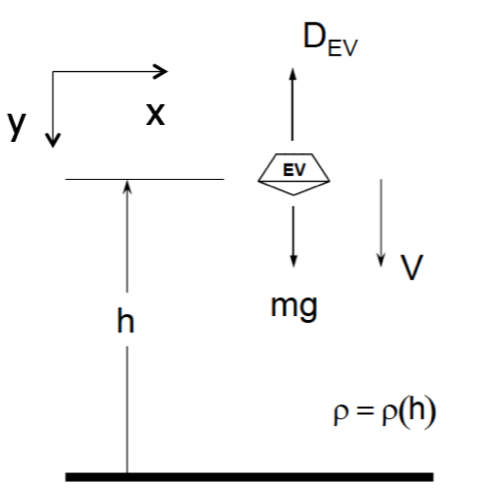
\includegraphics[scale=0.75]{FreeBodyDiagram.png} 
\end{figure}


\item
Known Values:\\
$D=2500N$\\
$T=0N$\\
$m=2196kg$\\
$g_m=3.96m/s^2$\\
$t = 5s$\\
\begin{equation}
\mathrm{m} \dot{\mathrm{V}}=\mathrm{D}+\mathrm{T}-\mathrm{mg_M}
\end{equation}
\begin{equation}
\frac{\mathrm{V}_{\mathrm{f}}-\mathrm{V}_{\mathrm{0}}}{\mathrm{t}}=-\frac{D}{m} - g_m
\end{equation}
\begin{equation}
\frac{\mathrm{V}_{\mathrm{f}}-(-100)}{\mathrm{5}}=-\frac{2500}{2196} - 3.96
\end{equation}

$V_f=-112.76 m/s$\\

Since the vehicle has a velocity towards the surface of Mars the sign of the component is negative. After the parachute gets released, the vehicle starts accelerating toward the surface of Mars which is why the velocity increases in a negative direction.

\item
To find the position after the vehicle free falls for 5 seconds after the parachute is released, integrate the acceleration formula twice to find the position. The constants when integrating are equal to the initial value (${\mathrm{V_0}}$ and $\mathrm{h_0})$.
\\\\
Known Values:
\\
$D=2500N$\\
$T=0N$\\
$m=2196kg$\\
$g_M = 3.96m/{s^2}$\\
$t = 5s$\\
$h_0=1800m$\\
$V_0=-112.76m/s$\\\\\\\\
\begin{equation}
\dot{\mathrm{V}}=\frac{\mathrm{D}}{\mathrm{m}}-\mathrm{g_M}\\
\end{equation}
\begin{equation}
{\mathrm{V}}=V0+\frac{\mathrm{D}}{\mathrm{m}}*t-\mathrm{g_M}*t
\end{equation}
\begin{equation}
h=h_0+V_0*t+\frac{1}{2}\frac{\mathrm{D}}{\mathrm{m}}*t^2-\frac{1}{2}\mathrm{g_M}*t^2
\end{equation}

$h=1268.01m$

\item
For this part, the vehicle has decelerated to a hovering position using the thrusts. The vehicle will stay in an equilibrium position to lower the rover to the surface of Mars. Since the vehicle used fuel to slow down to a hovering position, the mass at the beginning of the hovering phase is 1200 kg. Since the vehicle is no longer moving, the drag component and acceleration during this part is equal to zero newtons and metres per second respectively. The equation of motion for this portion of the flight is stated below.\\
\begin{equation}
\mathrm{T}-\mathrm{m*g_M}=0
\end{equation}
\begin{equation}
\mathrm{T}=\mathrm{m*g_M}=(1200)*(3.69)=4428 N
\end{equation}
\begin{equation}
Throttle_{setting}=\frac{T}{T_{Tot}}=\frac{4428}{4*3000}=0.1845=18.45\%
\end{equation}
\begin{equation}
\mathrm{I_{sp}}=\frac{T}{\dot{m}*g_0}
\end{equation}
\begin{equation}
\mathrm{\dot{m}}=\frac{T}{I_{sp}*g_0}=\frac{4428}{200*9.81}=2.26kg/s
\end{equation}
\begin{equation}
M_p=\dot{m}*t_{hover}=(2.26)*(13)=29.34 kg
\end{equation}

\item
In Part e of this problem, you can find the maximum acceleration error that will be produced having assumed that the mass remains constant by solving for the acceleration and inputting the mass as the total mass minus the mass of propellant used. This is the maximum acceleration error since the thrust used in this calculation will be the thrust needed to keep the initial mass at zero acceleration while using the final mass of the vehicle.
\begin{equation}
\dot{\mathrm{V}}=\frac{\mathrm{T}}{\mathrm{m}}-\mathrm{g_M}=\frac{\mathrm{4428}}{\mathrm{1200-29.34}}-\mathrm{3.69}=0.0925m/s^2
\end{equation}


\item
If the thrusters are not throttled to compensate for this change in mass error, the vehicle will accelerate upward away from the surface of Mars. The acceleration will start to increase from zero as the propellant mass is depleted.
\end{enumerate}